\documentclass[letterpaper, 10 pt, conference]{IEEEtran}
\IEEEoverridecommandlockouts
% The preceding line is only needed to identify funding in the first footnote. If that is unneeded, please comment it out.
\usepackage{cite}

\usepackage{subcaption}
\usepackage{multirow}% http://ctan.org/pkg/multirow
%\addbibresource{bibtex.bib}
\usepackage[table]{xcolor}
\usepackage{amsmath,amssymb,amsfonts}
\usepackage{algorithmic}
\usepackage{graphicx}
\usepackage{textcomp}
\usepackage{xcolor}
\usepackage[normalem]{ulem}
\def\BibTeX{{\rm B\kern-.05em{\sc i\kern-.025em b}\kern-.08em
    T\kern-.1667em\lower.7ex\hbox{E}\kern-.125emX}}


%% custom commands
\newcommand{\Rob}[1]{\textcolor{red}{(#1)}}
\newcommand{\Dan}[1]{\textcolor{blue}{(#1)}}
\newcommand{\Yves}[1]{\textcolor{brown}{(#1)}}

% use bold for vectors instead of arrows
\renewcommand{\vec}[1]{\boldsymbol{#1}}


\begin{document}


\title{A Proprioceptive Method for Soft Robots\\ Using Inertial Measurement Units%
% under the Piece-wise Constant Curvature Assumption %\\
%{\footnotesize \textsuperscript{*}Note: Sub-titles are not captured in Xplore and should not be used}
%\thanks{Identify applicable funding agency here. If none, delete this.}
}

\author{Yves J. Martin, Daniel Bruder, Robert J. Wood%
\thanks{This work was supported by a Space Technology Research Institutes
grant (number 80NSSC19K1076) from NASA’s Space Technology Research
Grants Program.}% <-this % stops a space
% \thanks{Yves J. Martin is \Dan{Yves you can fill in with institutional info about EPFL}.}% <-this % stops a space
\thanks{Yves J. Martin, Daniel Bruder, and Robert J. Wood are with the John A. Paulson School of Engineering and Applied Sciences, Harvard University, Cambridge, MA, 02138 USA (e-mail: yves@martin.yt, dbruder@seas.harvard.edu, rjwood@seas.harvard.edu).}% <-this % stops a space
}


\maketitle

\begin{abstract}
%% AIMS: What practical or theoretical problem does the research respond to, or what research question did you aim to answer?
Proprioception, or the perception of the configuration of one's body, is challenging to achieve with soft robots due to their infinite degrees of freedom and incompatibility with most off-the-shelf sensors. 
%
This work explores the use of inertial measurement units (IMUs), sensors that output orientation with respect to the direction of gravity, to achieve soft robot proprioception.
%
A simple method for estimating the shape of a soft continuum robot arm from IMUs mounted along the arm is presented.
The approach approximates a soft arm as a serial chain of rigid links, where the orientation of each link is given by the output of an IMU or by spherical linear interpolation of the output of adjacent IMUs.
%
In experiments conducted on a 660mm long real-world soft arm, this approach provided estimates of its end effector position with a median error of less than 10\% of the arm's length.
%
This demonstrates the potential of IMUs to serve as inexpensive off-the-shelf sensors for soft robot proprioception.


\end{abstract}

\begin{IEEEkeywords}
Modeling, Control, and Learning for Soft Robots; Kinematics; Sensor Fusion
\end{IEEEkeywords}
\section{Introduction}  \label{sec:introduction}

%% Soft robots are limited by lack of sensors
Proprioception, or the perception of the configuration of one's own body, is essential to robot planning and control.
The configuration of a rigid-bodied robot can be fully described by a finite set of joint displacements which are readily measured using off-the-shelf sensors such as joint encoders.
The configuration of a soft robot, however, is infinite dimensional and cannot readily be measured using off-the-shelf components.

%% Existing soft sensor technologies
To address this shortcoming, a number of sensing technologies have been developed specifically for soft robots \cite{wang2018toward}.
Flexible resistive sensors infer strain by measuring the change in resistance of channels filled with conductive liquids such as liquid metals \cite{park2012design, muth2014embedded} or ionic liquids \cite{helps2018proprioceptive}.
Flexible capacitive sensors estimate changes in geometry by measuring changes in capacitance of stretchable electrodes separated by an elastomeric dielectric layer \cite{yuen2018_strain}.
Optical strain sensors detect changes in geometry by measuring variations in intensity, frequency, or phase of light in a light transmission medium \cite{galloway2019_fiberopt, ZHUANG20187, zhao2016helping, van2018soft}.
Magnetic strain sensors infer displacement by measuring the response of a Hall effect sensor embedded in a soft medium relative to a fixed magnetic field \cite{luo2017_magnet, ozel2015precise}.
Inductive strain sensors estimate changes in geometry by measuring inductance variations caused by transducer mechanisms such as coil geometry and mutual inductance \cite{felt2015contraction, lazarus2018bubble, felt2019inductance}.
Deformable sensing fabrics or ``skins'' that incorporate several soft sensing technologies into a single versatile package have also been developed \cite{case2018_fabrics, Yuen2017_fabric}.

%% FIG: Overview
\begin{figure}
    \centering
    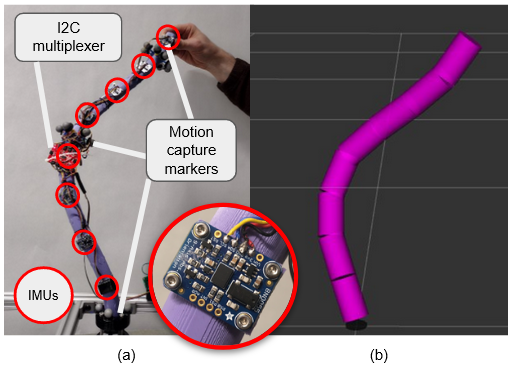
\includegraphics[width=\linewidth]{fig/schematic2.png}
    \caption{(a) The soft arm platform, with IMUs labeled, used to evaluate our estimation methods. (b) A serial-chain rigid-body model approximation of the soft arm motion is shown.}
    \label{fig:schematic}
\end{figure}

%% Current custom soft robot sensors have shortcomings
Each of these sensor types measure the strain of a flexible element.
Using strain measurements to construct an estimate of the pose of a soft arm requires integrating strain along the length, imposing accuracy limitations since small inaccuracies in strain along the length will compound into much larger pose errors.
Furthermore, while each sensor type has its own unique pros and cons, a common issue among them is nonlinear time-variant behavior and hysteresis.
This has motivated the use of machine learning techniques to identify the mapping from raw sensor output to deformation from data \cite{tapia2020_makesense, truby2020_piezo, thuruthel2019soft}.

%% Mocap is an okay alternative but has its own limitations
An alternative to embedded sensors is an external motion capture system.
Such systems utilize an array of externally-mounted infrared cameras to track the position of reflective markers in 3D space.
By coating a soft robot in reflective markers one can use motion capture data to estimate the robot’s shape.
Commercial motion capture systems offer an accurate and reliable method for sensing the deformation of soft robots, but they are expensive and impose severe restrictions on the environment in which a robot can operate.
Motion capture systems are not portable, are sensitive to lighting conditions, and are susceptible to errors due to occlusions, making it impossible to use them outside of a controlled laboratory setting.

%% Proposed solution: IMUs
This paper explores the use of Inertial Measurement Units (IMUs) for sensing the shape of continuum soft robots.
IMUs are off-the-shelf orientation sensors that combine a three-axis accelerometer, three-axis gyroscope, and three-axis magnetometer with an on-board sensor fusion algorithm.
Due to their extensive use in smartphones, tablets, and wearable fitness trackers, IMUs have become widely available and inexpensive, and there are many well-developed computational resources for integrating them into robotic systems \cite{ahmad2013reviews}.

%% Other papers that use IMUs for soft robots
Previous work has explored the use of IMUs for proprioception in soft robots.
In \cite{hughes2020sensing}, two IMUs were used in combination with motor encoders to estimate the pose of a single segment continuum body manipulator assuming constant curvature.
In \cite{yirmibesoglu2016hybrid} two IMUs were embedded into the ends of an elastomeric liquid metal strain sensor to form a hybrid sensor capable of measuring the angle of deflection of a soft bending actuator and the joint position of a rigid robot arm. 
In both of these cases, IMUs were combined with other sensor types (i.e. encoders, strain sensors) to estimate the pose of a one segment soft structure. 

%% Summary of contributions
The contribution of this paper is a simple method for estimating the shape of a full continuum arm using only IMUs.
The approach approximates the infinite-dimensional shape of a continuum arm with a finite-dimensional rigid-body model, and does not require any prior training.
In real-world validation experiments, it is shown to estimate end-effector position to within 10\% of arm length of median error, putting its accuracy on par with that of other soft sensors while avoiding the limitations imposed by external motion capture systems.

%% Outline of the rest of paper
The remainder of this paper is organized as follows.
Section \ref{sec:methods} describes how IMU data is utilized to construct an estimate of the shape of a robot arm.
Section \ref{sec:experiments} describes how the performance of the IMU-based sensing approach was evaluated on a real-world soft arm platform.
Section \ref{sec:results} presents the results of these experiments.
Section \ref{sec:discussion} discusses the results, likely sources of error, and potential improvements.
Section \ref{sec:conclusion} offers concluding remarks and proposes several avenues for future work.

\section{Methods}   \label{sec:methods}

IMU measurements provide the arm's orientation at given spots along the arm. 
This section will discuss how to use this data  to estimate the full arm shape using two different arm parametrizations.
For both of the presented models, the arm is parameterized as a series of rigid segments. 

In part \ref{rigid body model}, one segment per IMU is used. 
In part \ref{pseudo-PCC rigid body model}, we use spherical linear interpolation to create ``virtual IMUs" to increase the number of segments without increasing the number of IMUs. 
% This method approximates piece-wise constant curvature model (PCC).
In the limit, this method approximates a Piecewise Constant Curvature model (PCC) \cite{webster2010_pcc}. Both models are constructed from IMU orientation data in the form of quaternions, which are singularity free, as opposed to Euler angles which suffer from the Gimbal Lock issue \cite{doi:10.1177/003754976500400610}.
Quaternions are also broadly used in computer science and as a default IMU output format.

The models specify the shape of the arm as a collection of joint coordinates.
However, because both models represent the arm as a series of rigid segments, it is straightforward to compute the coordinates of any point along the length of the arm using linear interpolation between two adjacent joints.
% The formulas are given only for the edges of the segments, but it is easy to compute any data point along the arm using linear interpolation between the two adjacent edges. 

\subsection{Rigid-body model} \label{rigid body model}
% Here will be presented a mathematical model for Fig. \ref{models}(a)
The arm is modeled by $N+1$ straight links of length $L^R_i \text{, } i \in \{0,...,N\}$, called segments (see Fig.~\ref{models}(a)). 
An IMU is fixed to each segment, ideally on the center.
The $i^{th}$ segment is oriented along the IMU frame defined by its quaternion $\mathbf{q_i}$, $i \in \{0,...,N\}$ where
$\mathbf{q_0}$ is the orientation of the arm's base.
We define $R_q(\mathbf{q})$ as the 3x3 rotation matrix extracted from a quaternion $\mathbf{q} = a + i b + j c + k d$ \cite{tf_lib_ROS},

\begin{equation}
    R_q(\mathbf{q}) = \begin{pmatrix} 1 - 2(c^2+d^2) & 2(b c-a d) & 2(b d + a c) \\ 
    2(b c + a d) & 1 - 2(b^2 + d^2) & 2(c d - a b) \\
    2(b d - a c) & 2(c d + a b) & 1 - 2(b^2 + c^2) \end{pmatrix}
\end{equation}

Let $\mathbf{\hat{x}^{R}_i}$ be an estimate of the position of the joint between segment $i$ and segment $(i-1)$ according to this model.
It is computed by summing the displacements of the first $i-1$ links, according to the following expression,


\begin{equation}
    \mathbf{\hat{x}^{R}_i} =  \sum_{j=0}^{i-1} R_q(\mathbf{q_j}) \begin{pmatrix} 0 \\0 \\ L^R_j \end{pmatrix}
       \label{formula_rigid_body_model_2}
\end{equation}
Note that the superscript $(\cdot)^R$ denotes a variable related to the rigid-body model.

\subsection{PCC-extended rigid-body model} \label{pseudo-PCC rigid body model}

To make the rigid-body model smoother and more accurate, we divide each segment into $n$ sub-segments.
Each sub-segment orientation is computed under the assumption that the segment's curvature is constant.
As $n$ increases, this model approximates a PCC model.

Let us define $L^E_i$ as the distance between $\mathbf{q_i}$ and $\mathbf{q_{i+1}}$,
%
and $\mathbf{q_{i,k}}$ as the orientation quaternion of the $k^{th}$ sub-segment of the $i^{th}$ segment (see Fig.~\ref{models}(b)), which is computed using spherical linear interpolation between $\mathbf{q_i}$ and $\mathbf{q_{i+1}}$.

\begin{equation}
    \mathbf{q_{i,k}}=slerp\left(\mathbf{q_i},\mathbf{q_{i+1}},\frac{2k+1}{2n}\right)
\end{equation}
The function $slerp$ represents spherical linear interpolation \cite{fast_slerp} and is defined as,
\begin{equation}
slerp(\mathbf{q_a},\mathbf{q_b},t) = (\mathbf{q_b} \mathbf{q_a}^{-1})^t \mathbf{q_a}
\end{equation}
where $t \in [0,1]$ is the interpolation variable such that $slerp(\mathbf{q_a},\mathbf{q_b},0) = \mathbf{q_a}$ and $slerp(\mathbf{q_a},\mathbf{q_b},1) = \mathbf{q_b}$. \\

Next, the position of the $k^\text{th}$ joint of the $i^\text{th}$ segment, denoted $\mathbf{\hat{x}_{i,k}^E}$, is computed by summing the displacement of all preceding joints according to the following expression,
\begin{equation}
    \mathbf{\hat{x}_{i,k}^{E}} = \mathbf{\hat{x}_{i,0}^{E}} + \sum_{m=0}^{k-1} R_q(\mathbf{q_{i,m}})\begin{pmatrix} 0 \\0 \\  L^E_i/n \end{pmatrix} 
\end{equation}
Note that the superscript $(\cdot)^E$ denotes a variable related to the PCC-extended rigid-body model.
%

We define the $0^{th}$ joint of the $0^{th}$ segment to be located at the origin,
%
\begin{equation}
     \mathbf{\hat{x}_{0,0}^{E}} = \begin{pmatrix} 0 \\0 \\  0 \end{pmatrix} 
\end{equation}
and since the $n^{th}$ joint of segment $i$ is the same as the $0^{th}$ joint of segment $i+1$ the following are equivalent, 
%
\begin{equation}
   \mathbf{ \hat{x}_{i+1,0}^{E}} = \mathbf{\hat{x}_{i,n}^{E}}
\end{equation}
%


\begin{figure}
    \centering
    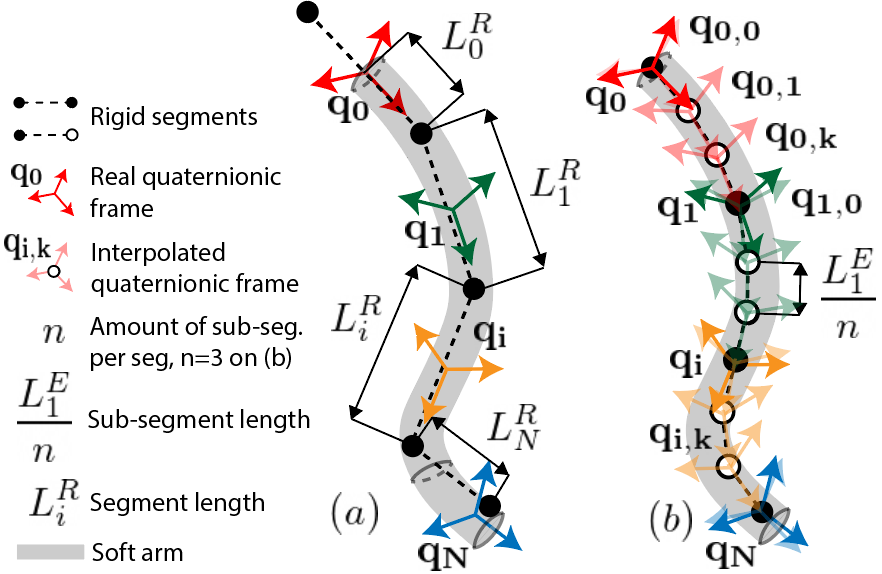
\includegraphics[width=\linewidth]{fig/models2.png}
    \caption{Different models to approximate the state of a soft continuum arm using IMUs: (a) rigid-body model, (b) and PCC-extended rigid-body model.}
    \label{models}
\end{figure}

\section{Experiments}   \label{sec:experiments}

\subsection{Description of continuum arm}

To validate the IMU-based modeling approach presented in Section~\ref{sec:methods}, we constructed a soft continuum arm and outfitted it with IMU sensors.
The arm is a cylinder of silicon (Smooth Sil 945) with a diameter of 25mm and of length 660mm. 
The structure is purely passive, it does not have any actuators.
Eight IMUs (bno055 Bosch) were evenly spaced along the length of the arm and fixed in place with screws into flat slots on the arm.
We selected this geometry to make the arm as flexible as possible while accommodating the 25x20mm footprint of the IMU breakout boards and allowing them to be spaced 80-100mm apart. Empirically, this spacing permits a maximum angle of $\pi/2$ between adjacent IMUs.
The update frequency of the IMUs is 31Hz, and they are read by an Arduino Mega 2560 using an I2C channel and an I2C multiplexer.
Two motion capture markers were fixed to the arm at lengths $M_1=360$mm and $M_2=600$mm.
There was only two motion capture markers because when we tried to use a higher density of markers, the motion capture system would mix up the markers.
The motion capture system (Vicon) has a precision of 1mm and an update frequency of 100Hz.

\subsection{Validation experiments: Motion capture vs. IMU model}
% \subsubsection{Outline of the validation experiments}
To evaluate the accuracy of our models, motion capture is used as ground truth.
While the arm is moved, measurements from the IMUs and the motion capture system are recorded. The IMU data is then used to construct models according to Section \ref{sec:methods} offline.
The positions of the motion capture markers are estimated from the models and compared to the actual positions recorded by the motion capture system.
In all experiments, error is defined as the Cartesian distance between the estimated positions of the motion capture markers and their actual positions.
To evaluate how model performance is affected by the density of IMUs along the arm, both models are constructed using the data from two, four, and eight IMUs.


\subsubsection{Rigid-body model experiment}
The rigid-body model is implemented using two, four, and eight IMUs (and thus with an equivalent number of segments). The position of the IMUs along the arm are shown in Table~\ref{tab:which IMUs}.
We set $L_0 = 0$mm since the first segment of length $L_0$ (see Fig \ref{models}) empirically induces a vertical error offset. 
When using two and four IMUs, the length of the arm can be divided into two and four equal sections, respectively, with an IMU mounted to the midpoint of each section.
For eight IMUs, when the length of the arm is divided into 8 equal sections, the segmentation is made such that the IMUs lie at the endpoints of the sections instead of the center due to their physical spacing.

\subsubsection{PCC-extended rigid-body model experiment}

The PCC-extended rigid-body model is tested w.r.t. two variables: the number of segments, and the number of IMUs.
First, we fixed the number of IMUs to the maximum, i.e. eight IMUs, and used 8, 16, 32, and 64 segments. 
Results shown in Fig.~\ref{fig:plateau} suggests that 16 segments are sufficient to approximate the maximum curvature exhibited by our arm.
% We interpret this as PCC model is approximated well enough by 16 sub-segments overall for the maximum curvature and the length of this arm. 
To explore the impact of the number of IMUs on pose estimation accuracy, we generated a 16 segments model using data from two, four, and eight IMUs.
% fixed the number of segments to 16 and we used 2, 4 and 8 IMUs to generate a 16 segment model.
The position of the IMUs used along the arm are shown in Table~\ref{tab:which IMUs}. Results shown in Fig.~\ref{fig:err_pcc16_model} indicate that even for the same number of segments (i.e., 16), the error decreases as the number of IMUs increases.

\begin{table}[ht]
    \centering
    \begin{tabular}{|c|c|m{9pt}|m{9pt}|m{9pt}|m{9pt}|m{9pt}|m{9pt}|m{9pt}|m{9pt}|}
        \hline
        IMU \# & Base* & 1 & 2 & 3 & 4 & 5 & 6 & 7 & 8  \\
        \hline
        \hline
        pos [mm] & 0 & 80 & 160 & 240 & 320 & 400 & 480 & 560 & 640 \\
        \hline
        2 IMUs & E &  & R &  & E &  & R &  & E \\
        \hline
        4 IMUs & E &  & X &  & X &  & X &  & X \\
         \hline
        8 IMUs & E & X  & X & X & X & X & X & X & X \\
        \hline       
    \end{tabular}
    \caption{This table shows which IMUs are selected for a given number of IMUs used to feed each model. Pos corresponds to the position of the IMU along the arm. ``R" stands for ``rigid-body only", ``E" stands for ``PCC-extended rigid-body model only", and ``X" stands for both. \\ *base is the orientation of the arm's base, not counted as an IMU but used in the PCC-extended rigid-body model.}
    \label{tab:which IMUs}
\end{table}

\subsubsection{Timing synchronization} To ensure the same sampling frequency on both the IMU model and motion capture signals, linear interpolation across time is processed on the model output. The time delay between both signals is computed using cross-correlation and removed. 

\subsection{Conditions of the data acquisition}

In a motion capture environment, the arm is fixed, base up, on an elevating structure (See Fig.~\ref{fig:schematic}).
Over a $250$sec trial, the arm is moved manually with a stick attached to the arm between the two motion capture markers. During the trial 8,000 samples are collected, 
% \sout{The flexibility of the stick makes the arm's movement smooth and fast:} 
The median of the arm's moving speed is $0.1$ms$^{-1}$ at marker 1 and $0.2$ms$^{-1}$ at marker 2, reaching speeds up to $0.6$ms$^{-1}$.

% The rigid fixation of the arm, heads up, results in a higher curvature at the bottom than at the top.

The arm is moved in different modes such as oscillating (going back and forth on each side of the structure, the tip reaching positions below the base w.r.t the z-axis), buckling (pseudo vertical position and contractions along the z-axis), and ``dog chasing its tail" (the arm making circles around the z-axis while its shape forms a question mark).


\section{Results}   \label{sec:results}

\subsection{Main takeaways} 

%% Relative error
\subsubsection{Overall estimation performance for both models}
The lowest error for the rigid-body model was found using eight IMUs with a median error of 48mm. 
The lowest error for the PCC-extended rigid-body model was found using eight IMUs with a median error of 37mm. 
As described in Table~\ref{tab:rel_arr_both_models}, the error normalized by the distance along the arm, which we refer to as \emph{relative error}, decreases from $L=360$mm to $L=600$mm for both models.
The PCC-extended rigid-body model is consistently more accurate than the rigid-body model, with approximately 25\% lower error.

\subsubsection{Computation considerations}
The rigid-body model can be computed in real time for two, four, and eight IMUs using a personal computer with an Intel® Core™ i7-10510U Processor (4.90 GHz) and 16GB of RAM.
The PCC-extended rigid-body model could not be constructed in real-time on the same machine, due to the added computational burden of repeatedly performing spherical linear interpolation. 
It took 18 minutes to compute each model for 4 min 10 secs of recording, which equates to roughly a factor of 4.4 slow-down relative to real time.
It should be noted, however, that a more efficient implementation could lower this computation time  significantly.

\begin{table}[]
    \centering
\begin{tabular}{|c|c|c|c|}

\hline
  Marker & Quartile & Rigid-body & PCC-extended \\

\hline
 M1 (L=360mm)  &  Median & 13.3\% &  10.2\% \\
\hline 
M1 (L=360mm) & $Q_3$ &17.7\% & 13.5\% \\
\hline
 M2 (L=600mm)   &  Median & 11.8\% & 9.1\% \\
\hline 
 M2 (L=600mm) & $Q_3$ & 16.25\% & 13.8\% \\
\hline
\end{tabular}
    \caption{Median and the third quartile (Q3) of the relative error for 16 segment models generated using
    % Error, w.r.t the position of the mocap marker,
    % of the rigid body model and the PCC-extended Rigid-body model 
    using eight IMUs.}
    \label{tab:rel_arr_both_models}
\end{table}

\subsection{Results for the rigid-body model} 

As expected, accuracy increases with the density of IMUs for both models. 
However, the accuracy doesn't increase linearly: for marker \#1, the median relative error for two, four, and eight IMUS is 44.4\%, 15.0\%, and 13.6\%, respectively (Fig. \ref{fig:err_rigid_boy_model}). 
Furthermore, the evolution of the relative error decreases along the arm. For eight IMUs at $L=360$mm, the relative error is 13.3\% whereas at $L=600$mm, the relative error is 11.5\% (Tab. \ref{tab:rel_arr_both_models}).

\begin{figure}[ht!]
    \centering
    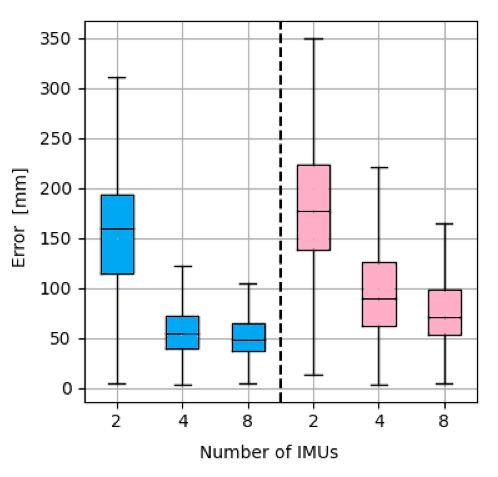
\includegraphics[width=\linewidth]{fig/error_RBM.png}
    \caption{Error of the rigid-body model with two, four, eight IMUs. The blue box-plots corresponds to the error on the marker 1. The pink box-plots corresponds to the error on the marker 2.}
    \label{fig:err_rigid_boy_model}
\end{figure}


\subsection{Results for the PCC-extended rigid-body model} 

The PCC-extended rigid-body model has two parameters to define: the number of segments and the number of IMUs. 
We will first present the effects of changing the number of segments using eight IMUs, and then present the effects of changing the number of IMUs using 16 segments.

\subsubsection{Effects of changing the number of segments using eight IMUs (Fig.~\ref{fig:plateau})}

The accuracy of the model increases with the number of segments until a plateau is reached. 
For example, while the Q3 of the error for eight segments is 16.9\%, for 16 segments and more, the Q3 of the error remains similar at 13.5\%.

\begin{figure}[ht!]
    \centering
    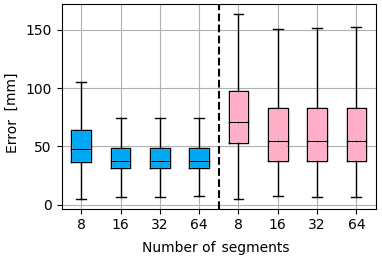
\includegraphics[width=\linewidth]{fig/plateau.png}
    \caption{Using PCC-extended rigid-body model with eight IMUs and 8, 16, 32, and 64 segments. The blue box-plots corresponds to the error on the marker 1. The pink box-plots corresponds to the error on the marker 2.}
    \label{fig:plateau}
\end{figure}

\subsubsection{Effects of changing the number of IMUs using 16 segments (Fig.~\ref{fig:err_pcc16_model})}

Similar to the rigid-body model, error decreases as the number of IMUs increases. However, unlike the rigid-body model, the error continues decreasing significantly between four and eight IMUs. The median of the relative error decreases by 10\% between markers 1 and 2. 

\begin{figure}[ht!]
    \centering
    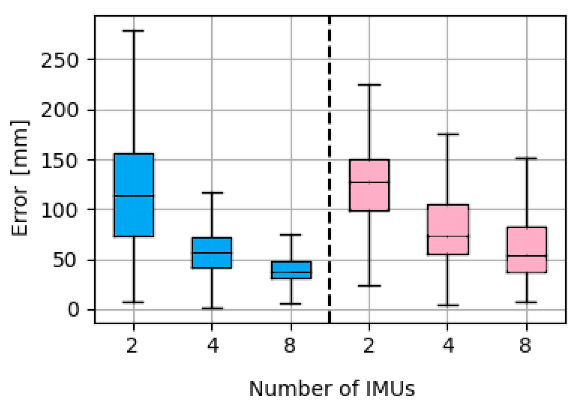
\includegraphics[width=\linewidth]{fig/pcc16.png}
    \caption{Error of the 16 segments PCC-extended rigid-body model with two, four, and eight IMUs. The blue box-plots corresponds to the error on the marker 1. The pink box-plots corresponds to the error on the marker 2.}
    \label{fig:err_pcc16_model}
\end{figure}

\subsubsection{The error in pose estimation along the arm}
% Computing values
The absolute error increases along the length of the arm. For eight IMUs and 16 segments, at $L=360$mm, the Q3 of the absolute error is $48$mm whereas at $L=600$mm, the Q3 of the absolute error is $83$mm (Tab. \ref{tab:rel_arr_both_models}).
Fig \ref{fig:hull} shows a 3D hull containing the Q3 of the PCC-extended rigid-body model estimation.

However, if we consider the error normalized by the length moving from the base along the arm, the relative error decreases. For eight IMUs and 16 segments, at $L=360$mm, the Q3 of the relative error is 10.2\% whereas at $L=600$mm, the Q3 of the relative error is 9.1\% (Tab. \ref{tab:rel_arr_both_models}).

\begin{figure}
    \centering
    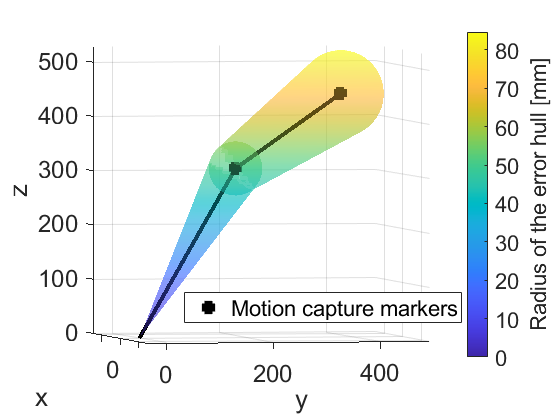
\includegraphics[width=\linewidth]{fig/hull2.png}
    \caption{3D hull containing 75\% of the PCC-extended rigid-body model estimation (error below the Q3) for eight IMUs and 16 segments. The arm pose is reconstructed using motion capture data. }
    \label{fig:hull}
\end{figure}







\section{Discussion} \label{sec:discussion}

% \subsection{Likely causes of error and openings for improvement}    %% Don't need subsections here
A likely cause of error for the rigid-body model is the length of the segments for high bending values. 
Bending reduces the distance between the joints, whereas the rigid-body model keeps it constant.
%
The PCC-extended rigid-body model captures the overall shape better, but since the model is a serial chain, a small error near the base propagates through the entire arm.
This is why the error at the end-effector tends to be larger than that at the motion capture marker near the middle of the arm (see Fig.~\ref{fig:hull}).
% Future work could investigate using non-uniform distributions of IMUs to increase sensitivity in regions with the most expected bending.

Another likely source of error is the orientation of the arm relative to gravity.
In our experiments the arm was mounted such that it points upwards from the base, causing the weight of the arm to induce larger non-constant curvatures near the base.
This curvature near the base leads to errors that propagate and grow along the length of the arm.
% The heads up position of the arm tends to show non-PCC behavior of the arm, which would explain the error. 
We could potentially reduce this error by mounting the arm such that it points downward instead, 
% it the arm heads down would probably increase highly the accuracy of the system, typically in an industrial context.
or by changing the IMU positions along the arm such that the density of IMUs increases as we get closer to the arm's base.

IMU drift might also generate errors in the IMU measurements, especially at the base. 
The IMU we used, the bno055, auto-calibrates in the background by reaching different positions \cite{sensortec2016bno055}.
The first IMUs along the arm have a limited range of positions, which might reduce the quality of their calibration and therefore increase the error.

Ideally, the shape of the arm would be computed from IMU data quickly enough to provide a feedback signal to a real-time closed-loop controller.
In our experiments the rigid-body model was able to provide estimates in real-time, but the PCC-extended rigid-body model was not.
Because this work is meant only to be a proof of concept for IMU based proprioception, achieving real-time computation was not our focus.
However, there are many ways in which computational efficiency could be improved in the future.
% The study is meant to be a proof of concept: though, computational efficiency could be improved to have PCC-Extended Rigid-Body model running online. 
One such approach could be to ignore the real part of the quaternions and keep only a vector along which the arm would be aligned. 
Then linear interpolation could be used between these vectors, which is computationally 3 times lighter than spherical linear interpolation using MATLAB implementation \cite{matlab}. 


% \subsection{How many IMUs are needed for a given arm with the Rigid-body model?}     %% Don't need subsections here

Fig.~\ref{fig:err_pcc16_model} shows that increasing the number of actual IMU sensors used to generate a 16 segment model reduces the model's error. However, Fig. \ref{fig:plateau} shows that increasing the number of segments beyond 16 does not noticeably reduce the error. We interpret this to mean that a 16 segment rigid-body model is a suitable approximation of a PCC model of this arm.
% Therefore, we expect that 16 is the maximum number of IMUs needed to approximate the shape of the arm as accurately as a PCC model.
Therefore, we expect that for 16 or more IMUs, a rigid-body model and a continuous PCC model will approximate the shape of the arm with roughly equal accuracy.
This ``maximum number of IMUs'' will vary from arm to arm depending on its geometry and bending stiffness.
Future work could develop a method to compute this number for any soft arm as a function of its maximum curvature and some tolerated error threshold.
There are computation concerns when adding additional IMUs, however. Adding more IMUs could reduce the reading frequency, especially if using a Micro Controller Unit. This could be compensated by using higher speed protocols than I2C such as SPI.

%% Old version
% This sufficient approximation number of segments value could be used as the number of IMUs that should be used to estimate the state of a given arm at best, for instance using the rigid-body model. \Yves{I don't like this sentence, we should explain better why if you can't reduce the error with more segments, then why would you reduce the error with more IMUs?}
% . 
% This method could also be generalized to compute the number of required segments to model any soft arm, w.r.t its maximum curvature and the tolerated error in future work.







\section{Conclusion}    \label{sec:conclusion}

In this paper we show that IMUs -- inexpensive, available off-the-shelf, and easy-to-integrate -- can be used for proprioception of soft robot arms.
Using a rigid-body model generated from IMU data and spherical linear interpolation, we were able to estimate the position of the end-effector of a soft robot arm with a median error of less than 10\% of the arm's length.
% reaching the performance of a median error below 10\%. 
Future work could employ methods to improve the accuracy of IMU-based shape estimates.
Future work could also investigate ways to make IMUs easier to integrate into soft robots.
This could be done by mounting the IMUs on small custom PCBs, and by integrating an entire string of IMUs as a self-contained sensor.
% Eventually, this 1D model could even be extended to a 2D surface sensing, by mapping the target with IMUs along two dimensions instead of one. \Dan{elaborate a little further, or cut this part}.\Yves{is ok?}


\bibliography{bibli} 
\bibliographystyle{ieeetr}

\end{document}
